\documentclass[12pt]{article}
\usepackage{light}

\hidesolutions
%\showsolutions

\begin{document}

\recitation{5}{September 24, 2010}

\insolutions{
\section{Exponentiation and Modular Arithmetic}

Recall that RSA encryption and decryption both involve
exponentiation. To encrypt a message $m$, we use the following
equation:
\[
m' = \rem(m^e,n) \equiv m^e \pmod{n}.
\]
\noindent
And to decrypt a message $m'$, we use
\[
m = \rem((m')^d, n) \equiv (m')^d \pmod{n}.
\]
In practice, $e$ and $d$ might be quite large. But even for relatively
small values of these variables, the quantities $m^e$ and $(m')^d$ can
be very difficult to compute directly. Fortunately, there are
tractable and efficient methods for carrying out exponentiation of
large integer powers modulo a number. 

Let's say we are trying to encrypt a message. First, note that:
\begin{align*}
\rem(a\cdot b,c) & \equiv a \cdot b \pmod{c} \\
& \equiv \rem(a,c) \cdot \rem(b,c) \pmod{c} \\
& = \rem((\rem(a,c)\cdot\rem(b,c)) , c)
\end{align*}
This principle extends to an arbitrary number of factors, such that:
\begin{align*}
a_1\cdot a_2 \cdot \ldots \cdot a_n \equiv \rem(a_1,c)\cdot \rem(a_2,c)\cdot \ldots \cdot \rem(a_n,c) \pmod{c}
\end{align*}

\noindent
We illustrate this point with an example:

\noindent
\textbf{Example:} Find $\rem(23 \cdot 61 \cdot 19, 17)$.

We could find the remainder of $23 \cdot 61 \cdot 19 = 26657$ divided by $17$, but that would be a lot of unnecessary work! Instead, we notice the fact that $23 \equiv 6 \pmod{17}$, $61 \equiv 10 \pmod{17}$, and $19 \equiv 2 \pmod{17}$. Therefore, $23 \cdot 61 \cdot 19 \equiv 6 \cdot 10 \cdot 2 \pmod{17}$.

Similarly, we can reduce the remainder of $6 \cdot 10 \cdot 2$ divided by $17$. We notice the fact that $10 \cdot 2 = 20 \equiv 3 \pmod{17}$, so $6 \cdot 10 \cdot 2 \equiv 6 \cdot 3 = 18 \equiv 1 \pmod{17}$. We could have also calculated $6 \cdot 10 = 60 \equiv 9 \pmod{17}$ to get the same answer $6 \cdot 10 \cdot 2 \equiv 9 \cdot 2 = 18 \equiv 1 \pmod{17}$. While both methods here were relatively simple to use, how you choose to associate your factors may sometimes greatly affect the difficulty of a calculation!

\noindent
Let's return to RSA. Here's one way we might go about encrypting our message (though in a minute we'll consider a more efficient technique). We can compute $m=\rem(m^e,n)$ by breaking the exponentiation into a sequence of $e-1$ multiplications. We then take the remainder after dividing by $n$ after each one of these multiplications.

\noindent
\textbf{Example:} Encrypt the message $m=5$ with $e=6$ and $n=17$.

We are trying to find $\rem(m^e, n)$. We know that $m^{e} = 5^{6} = 5 \cdot 5 \cdot 5 \cdot 5 \cdot 5 \cdot 5$.  
\begin{align*}
5^2 \equiv 8 \pmod{17} \\
5^3 \equiv 8 \cdot 5 \equiv 6 \pmod{17} \\
5^4 \equiv 6 \cdot 5 \equiv 13 \pmod{17} \\
5^5 \equiv 13 \cdot 5 \equiv 14 \pmod{17} \\
5^6 \equiv 14 \cdot 5 \equiv 2 \pmod{17}
\end{align*}

\noindent
OK, that's nice, but for large $e$, $e-1$ is still a lot of multiplications! As we promised earlier, there's a yet more efficient way to do the exponentiation. It's called {\em repeated squaring}.

\noindent
\textbf{Example:} Encrypt a message $m=5$ with $e=149$ and $n=17$.

Note that the binary expansion of $149$ is $10010101$, so one can compute $\rem(5^{149},17)$ by computing $\rem(5^{128+16+4+1},17)$.
\begin{align*}
5^2 \equiv 8 \pmod{17} \\
5^4 \equiv 8 \cdot 8 \equiv 13 \pmod{17} \\
5^8 \equiv 13 \cdot 13 \equiv 16 \pmod{17} \\
5^{16} \equiv 16 \cdot 16 \equiv 1 \pmod{17} \\
5^{32} \equiv 1 \cdot 1 \equiv 1 \pmod{17} \\
5^{64} \equiv 1 \cdot 1 \equiv 1 \pmod{17} \\
5^{128} \equiv 1 \cdot 1 \equiv 1 \pmod{17}
\end{align*}

We used only 7 multiplications to find the remainders of $5^{2k} \pmod{17}$ by repeatedly squaring each previous output and taking the remainder.  Then, with only $3$ additional
multiplications to combine these products, we can compute $5^{128} \cdot 5^{16} \cdot 5^4 \cdot 5^1 \equiv 1 \cdot 1 \cdot 13 \cdot 5 \equiv 14 \pmod{13}$. This saved us $(149-1)-(7+3) = 138$ multiplications!

You may notice that in this particular case, $5^{16} \equiv 1 \pmod{17}$, so we could have even stopped our squaring at $5^{16}$ and reduced the problem to computing $\rem(5^{16 \cdot 9 + 4 + 1},17) \equiv (5^{16})^{9} \cdot 5^4 \cdot 5 \equiv 1^{9} \cdot 13 \cdot 5 \equiv 14 \pmod{17}$. For this we only needed $(4+2) = 6$ multiplications!

You may find this technique very useful in the next problem.
\newpage
}

\section{RSA: Let's try it out!}
You'll probably need extra paper.  \textit{Check your work carefully!}
\begin{enumerate}

\item 
As a team, go through the \textbf{beforehand} steps.
\begin{enumerate}

\item
Choose primes $p$ and $q$ to be relatively small, say in the
range 5-15.  In practice, $p$ and $q$ might contain several hundred
digits, but small numbers are easier to handle with pencil and paper.

\solution{We choose $p=7$ and $q=11$ for our example.}

\item
Calculate $n=pq$. This number will be used to encrypt and decrypt your messages.

\solution{In our example, $n=pq=77$.}

\item
Find an $e>1$ such that $\gcd(e, (p-1)(q-1)) = 1$.

The pair $(e,n)$ will be your \textit{public key}. This value will be broadcast to other groups, and they will use it to send you messages.

\solution{In our example, $p-1=6=2\cdot 3$ and $q-1=10=2\cdot 5$. Therefore, any $e$ that is odd and neither a multiple of 5 nor 3 would work. We choose $e=13$.}

\item Now you will need to find a $d$ such that $de \equiv 1 \pmod{(p-1)(q-1)}$.

\begin{itemize}
\item
Explain how this could be done using the Pulverizer. (Do not carry out the computations!)
\end{itemize}

\solution{ We can rewrite the equation $de \equiv 1 \pmod{(p-1)(q-1)}$ to read $de-1 = k(p-1)(q-1)$ for some integer value $k$. Rearranging this yields the equation $de-k(p-1)(q-1)=1$. Because $gcd(e,(p-1)(q-1))=1$, we know such a linear combination of $e$ and $(p-1)(q-1)$ exists! Using the Pulverizer will give us the coefficient $d$, and then we can adjust $d$ to be positive using techniques from class. In this case $d=-23$, which can be adjusted to $37$.}

\begin{itemize}
\item Find $d$ using Euler's Theorem given in yesterday's lecture.

The pair $(d,n)$ will be your \textit{secret key}. Do not share this with anybody!
\end{itemize}
 
\solution{
Since $e$ and $(p-1)(q-1)$ are relatively prime, we can claim by Euler's Theorem that $e^{\phi((p-1)(q-1))}\equiv 1 \pmod{(p-1)(q-1)}$ and hence $e^{\phi((p-1)(q-1))-1}\cdot e \equiv 1 \pmod{(p-1)(q-1)}$.
\\

This means $d=e^{\phi((p-1)(q-1))-1}$ is an \textit{inverse} of $e \pmod{(p-1)(q-1)}$. To find the value of $d$, we first calculate $\phi((p-1)(q-1))$. In our example, the factorization of $(p-1)(q-1)$ is $2^{2} \cdot 3 \cdot 5$, so $\phi((p-1)(q-1)) = (2^{2}-2^{1})(3^{1}-3^{0})(5^{1}-5^{0}) = 2 \cdot 2 \cdot 4 = 16$. We substitute $e$ and $\phi((p-1)(q-1))$ into our equation to get $d=13^{16-1}=13^{15}$.
\\

$13^{15}$ is a huge number! Therefore, we must reduce $d$ to something more manageable using \textit{repeated squaring}. In our example, we square $13$ to get $13^{2} = 169 \equiv 49 \pmod{60}$. We square our result to get $13^{4} = (13^{2})^{2} \equiv 49^{2} = 2401 \equiv 1 \pmod{60}$.
\\

Once we know $13^{4} \equiv 1 \pmod{60}$, our job is much easier. $13^{15} = (13^{4})^{3} \cdot 13^{2} \cdot 13 \equiv 1^{3} \cdot 49 \cdot 13 = 637 \equiv 37 \pmod{60}$. This matches our answer from the Pulverizer. Which method is easier depends on the particular numbers that we've chosen.
}

\end{enumerate}

When you're done, write your public key and group members' names on the board.

\item Now ask your recitation instructor for a message to encrypt and
  send to another team using \textit{their} public key.

  %\insolutions{ 

The messages $m$ correspond to statements from the codebook below:

\begin{enumerate}

\item[] 2 = Greetings and salutations!

\item[] 3 = Wassup, yo?

\item[] 4 = You guys are slow!

\item[] 5 = All your base are belong to us.

\item[] 6 = Someone on {\em our} team thinks someone on {\em
your} team is kinda cute.

\item[] 7 = You are the weakest link.  Goodbye.

\end{enumerate}
%} %end insolutions


\item \textbf{Encode} the message you were given using another team's
  public key.

\solution{Let's say our message was $m=3$ and the other team's public key was $(e,n) = (11,35)$. The encrypted message would then be $m' = \rem (3^{11},35)$. Using repeated squaring, we see that $3^{11}=3^{8+2+1}$. We compute $3^{2} = 9 \pmod{35}$, $3^{4} = 81 \equiv 11 \pmod{35}$, $3^{8} = (3^{4})^{2} \equiv 11^{2} = 121 \equiv  16 \pmod{35}$. Therefore $3^{11} \equiv 16 \cdot 9 \cdot 3 = 432 \equiv 12 \pmod{35}$, so our message is $m'=12$.}

\item Now \textbf{decrypt} the message sent to you and verify that you
  received what the other team sent!

\solution{Let's say the other team sent you the encrypted message $m'=26$. In our case, our private key was $(d,n) = (37,77)$. The decrypted original message would then be $m = \rem (26^{37},77)$. Using repeated squaring, we find $m=5$.}

\item 
Explain how you could read messages encrypted with RSA if you
could quickly factor large numbers.

\solution{Suppose you see a public key $(e, n)$.  If you can factor
  $n$ to obtain $p$ and $q$, then you can compute $d$ using the
  Pulverizer or Euler's Theorem.  This gives you the secret key $(d,
  n)$, and so you can decode messages as well as the intended
  recipient.}

\end{enumerate}

%%%%%%%%%%%%%%%%%%%%%%%%%%%%%%%%%%%%%%%%%%%%%%%%%%%%%%%%%%%%%%%%%%%%%%%%%%%%%%%

\textbox{
\begin{center}
RSA Public-Key Encryption
\end{center}

\begin{description}

\item[Beforehand] The receiver creates a public key and a secret key
as follows.

\begin{enumerate}

\item Generate two distinct primes, $p$ and $q$.

\item Let $n = pq$.

\item Select an integer $e$ such that $\gcd(e, (p-1)(q-1)) = 1$.\\ The
{\em public key} is the pair $(e, n)$.  This should be distributed
widely.

\item Compute $d$ such that $de \equiv 1 \pmod{(p-1)(q-1)}$.\\ The
{\em secret key} is the pair $(d, n)$.  This should be kept hidden!

\end{enumerate}

\item[Encoding] The sender encrypts message $m$ to produce $m^\prime$ using
the public key:

\[
m' = \rem(m^e,n)
\]

\item[Decoding] The receiver decrypts message $m'$ back to message $m$
using the secret key:
\[
m = \rem((m')^d, n).
\]

\end{description}
}
\vfill\mbox{}


%% \newpage

%% \section{}

%% Many assertions about the real numbers have analogues in the integers
%% modulo a prime.  Here is an example.  Two nonparallel lines in the
%% real plane intersect at a point.  Algebraically, this means that the
%% equations
%% %
%% \begin{align*}
%% y & = m_1 x + b_1 \\
%% y & = m_2 x + b_2
%% \end{align*}
%% %
%% have a unique solution $(x, y)$, provided $m_1 \neq m_2$.  This
%% statement would be false if we restricted $x$ and $y$ to the integers,
%% since the two lines could cross at a noninteger point:

%% \begin{center}
%% \resizebox{!}{1in}{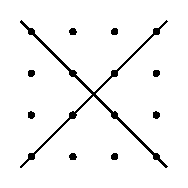
\includegraphics{integerlines.pdf}}
%% \end{center}

%% However, an analogous statement holds if we work over the integers
%% {\em modulo a prime $p$}.  Find a solution to the congruences
%% %
%% \begin{align*}
%% y & \equiv m_1 x + b_1 \pmod{p} \\
%% y & \equiv m_2 x + b_2 \pmod{p}
%% \end{align*}
%% %
%% of the form $x \equiv ? \pmod{p}$ and $y \equiv ? \pmod{p}$ where the
%% ?'s denote expressions involving $m_1$, $m_2$, $b_1$, and $b_2$.  You
%% may find it helpful to solve the original equations over the reals
%% first.

%% \solution{Subtracting the second congruence from the first, we have:
%% %
%% \begin{align*}
%% 0 & \equiv m_1 x+b_1 - (m_2 x + b_2)  \pmod{p} \\
%% (m_1 - m_2)x & \equiv b_2 - b_1 \pmod{p} \\
%% x & \equiv (m_1 - m_2)^{-1} \cdot (b_2 - b_1) \pmod{p}
%% \end{align*}
%% %
%% Substituting this value of $x$ into the first congruence, we have
%% %
%% \[
%% y \equiv m_1 \cdot (m_1 - m_2)^{-1} \cdot (b_2 - b_1) + b_1 \pmod{p}
%% \]
%% }


\end{document}
